\documentclass[2pt, a4paper, fleqn]{extarticle}

\usepackage[T2A]{fontenc}
\usepackage[utf8]{inputenc}
\usepackage[english,russian]{babel}
\usepackage{url}
%\usepackage{pscyr}

%\renewcommand{\rmdefault}{ftm}
\usepackage{setspace}
\onehalfspacing

\usepackage{changepage}
\usepackage{indentfirst} %первый абзац
%%\usepackage{moreverb}
\usepackage[noend]{algorithmic}
\usepackage{amssymb, amsmath, multicol,amsthm}
%%
\usepackage{enumitem, multicol}
\usepackage{titleps,lipsum}
%%
\usepackage{mathrsfs}
\usepackage{verbatim}
\usepackage{pb-diagram}
\usepackage{graphicx}
\graphicspath{ {images/} }
\usepackage{wrapfig}
\usepackage{xcolor}
\definecolor{new}{RGB}{255,184,92}
\definecolor{news}{RGB}{112,112,112}
\usepackage{wallpaper}
\usepackage{float}
\usepackage{hyperref}
\hypersetup{
%colorlinks=true,%
%linkcolor=news,%
linkbordercolor=new,
}



\usepackage{geometry}
\geometry{top=1cm,bottom=2cm,left=1cm,right=1cm}

%\flushbottom
%\ruggedbottom

\binoppenalty=5000
\parindent=0pt

\newcommand{\EDS}{\ensuremath{\mathscr{E}}}
\newcommand*{\hm}[1]{#1\nobreak\discretionary{}%
{\hbox{$\mathsurround=0pt #1$}}{}}
\newcommand{\divisible}{\mathop{\raisebox{-2pt}{\vdots}}}
\renewcommand{\theequation}{\arabic{equation}}
\def\hm#1{#1\nobreak\discretionary{}{\hbox{$#1$}}{}}
\newcommand{\bbskip}{\bigskip \bigskip}



%%\DeclareMathOperator{\tg}{tg}
%%\DeclareMathOperator{\ctg}{ctg}

\let\leq\leqslant
\let\geq\geqslant



% Remove brackets from numbering in List of References
\makeatletter
\renewcommand{\@biblabel}[1]{\quad#1.}
\makeatother

\begin{document}

\begin{center} {\Large Задача без смешанной производной второго шага. Постановка граничных условий в околополюсных точках.} \end{center}

Рассматривается уравнение, решаемое на втором шаге расщепления, без учёта смешанной производной: $$\dfrac{\partial n}{\partial t} = \dfrac{1}{a\cos\varphi} \dfrac{\partial }{\partial \varphi}\left[\dfrac{D}{a}\cdot(\cos^2  I \cos\varphi)\cdot\dfrac{\partial n}{\partial \varphi} - u\cdot(\sin I \cos I \cos\varphi)\cdot n \right] =  \dfrac{1}{\cos\varphi} \dfrac{\partial }{\partial \varphi}\left[\dfrac{D}{a^2}A(\varphi)\dfrac{\partial n}{\partial \varphi} - \dfrac{u}{2a}B(\varphi) n \right].$$

В этом уравнении $I = \arctg(2\tg \varphi)$, а функции $A(\varphi)$ и $B(\varphi)$ определены выражениями: $$A(\varphi) = \cos \varphi \cdot \cos^2(\arctg(2\tg \varphi)) = \dfrac{\cos\varphi}{1+4\tg^2\varphi}\mbox{ и }B(\varphi) = \cos\varphi \cdot \sin(2\arctg(2\tg \varphi))=\dfrac{4\sin\varphi}{1+4\tg^2\varphi}.$$

Необходимо аппроксимировать уравнение в околополюсных точках на сетке по переменной $\varphi$: узлы имеют номера от $1$ до $N_\varphi = 180$, $j = 1$ соответствует $\varphi = -89{,}5^\circ$, а $j = N_\varphi$ соответствует $\varphi = + 89{,}5^\circ$. Общая формула для узлов: $\varphi_j = -90^\circ + (j-0{,}5)\cdot 1^\circ$.



Графики функций $A$ и $B$ приведены ниже: 

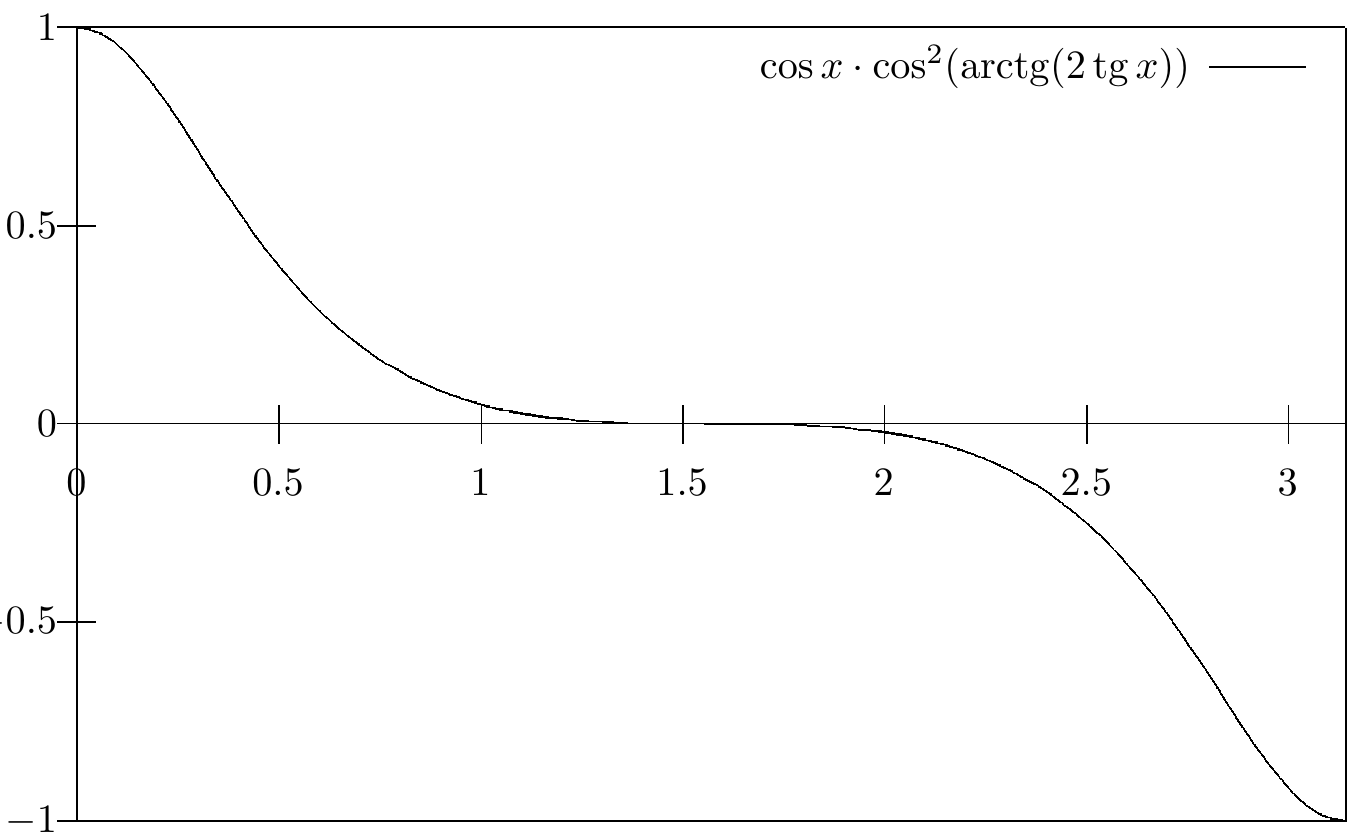
\includegraphics[scale=0.25]{A}

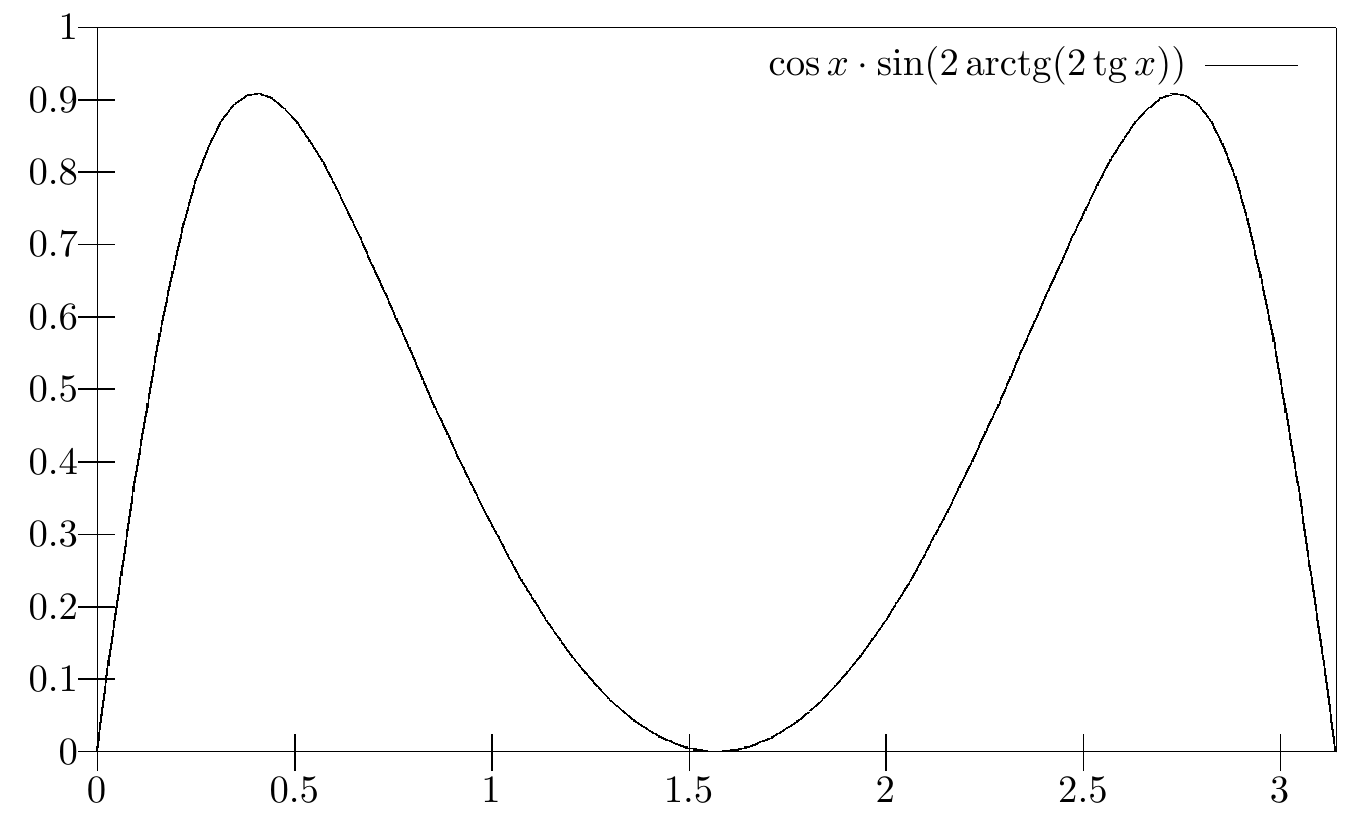
\includegraphics[scale=0.25]{B}

Имеют место следующие разложения при $\varphi\rightarrow\dfrac{\pi}{2}$: $$A(\varphi)=-\dfrac{1}{4}\cdot\left(\varphi-\dfrac{\pi}{2}\right)^3-\dfrac{1}{16}\cdot\left(\varphi-\dfrac{\pi}{2}\right)^5+o\left(\left(\varphi-\dfrac{\pi}{2}\right)^6\right); B(\varphi) = 1\cdot\left(\varphi-\dfrac{\pi}{2}\right)^2-\dfrac{1}{12}\cdot \left(\varphi-\dfrac{\pi}{2}\right)^4+o\left(\left(\varphi-\dfrac{\pi}{2}\right)^5\right)$$

Соответственно, при $x\rightarrow-\dfrac{\pi}{2}$: $$A(\varphi)=\dfrac{1}{4}\cdot\left(\varphi+\dfrac{\pi}{2}\right)^3+\dfrac{1}{16}\cdot\left(\varphi+\dfrac{\pi}{2}\right)^5+o\left(\left(\varphi+\dfrac{\pi}{2}\right)^6\right); B(\varphi) = -1\cdot\left(\varphi+\dfrac{\pi}{2}\right)^2+\dfrac{1}{12}\cdot \left(\varphi+\dfrac{\pi}{2}\right)^4+o\left(\left(\varphi+\dfrac{\pi}{2}\right)^5\right)$$

Для уравнения используем следующую схему:
$$\dfrac{n_{i,j}^{t+1}-n_{i,j}^t}{\tau} = \dfrac{1}{\cos\varphi_j} \bigg[\dfrac{D}{a^2}\left(A(\varphi_{j+1/2})\dfrac{n_{i, j+1}^{t+1}-n_{i,j}^{t+1}}{\Delta\varphi^2}-A(\varphi_{j-1/2})\dfrac{n_{i,j}^{t+1}-n_{i,j-1}^{t+1}}{\Delta\varphi^2}\right)-$$ $$-\dfrac{u}{2a}\left(\dfrac{B(\varphi_{j+1})n_{i,j+1}^{t+1}-B(\varphi_{j-1})n_{i,j-1}^{t+1}}{2\Delta\varphi}\right)\bigg]$$

\medskip

Рассмотрим границу $j = 1$, соответствующую южному полюсу и узлу $\varphi_j = - 89{,}5^\circ$. В этой точке поставим следующее условие: полный поток в разностной схеме равен нулю. Это означает, что $$\bigg[\dfrac{D}{a^2}\left(A(\varphi_{j-1/2})\dfrac{n_{i, j}^{t+1}-n_{i,j-1}^{t+1}}{\Delta\varphi^2}\right)-\dfrac{u}{2a}\left(\dfrac{B(\varphi_{j-1})n_{i,j-1}^{t+1}+B(\varphi_{j})n_{i,j}^{t+1}}{2\Delta\varphi}\right)\bigg) \bigg] = 0$$ В этом случае решается уравнение $$\dfrac{n_{i,j}^{t+1}-n_{i,j}^t}{\tau} = \dfrac{1}{\cos\varphi_j} \bigg[\dfrac{D}{a^2}\left(A(\varphi_{j+1/2})\dfrac{n_{i, j+1}^{t+1}-n_{i,j}^{t+1}}{\Delta\varphi^2}\right)-\dfrac{u}{2a}\left(\dfrac{B(\varphi_{j+1})n_{i,j+1}^{t+1}+B(\varphi_{j})n_{i,j}^{t+1}}{2\Delta\varphi}\right)\bigg) \bigg]$$

Заметим, что в отличие от значения функции $A$ в полуцелом узле, выражение $\dfrac{B(\varphi_{j-1})n_{i,j-1}^{t+1}+B(\varphi_{j})n_{i,j}^{t+1}}{2\Delta\varphi}$ не равно нулю в точности: подстановка значений $B$ с учётом приведенной выше асимптотики даёт $$\dfrac{B(\varphi_{j-1})n_{i,j-1}^{t+1}+B(\varphi_{j})n_{i,j}^{t+1}}{2\Delta\varphi\cos\varphi} \approx \dfrac{n}{2\Delta\varphi^2}\left[\left(\dfrac{\pi}{2} + \dfrac{\Delta\varphi}{2}-\dfrac{\pi}{2}\right)^2+\left(\dfrac{\pi}{2} - \dfrac{\Delta\varphi}{2}-\dfrac{\pi}{2}\right)^2\right] \approx \dfrac{n}{4}$$

Эта константа не зависит от $\Delta\varphi$, что приводит к <<скачкам>> в околополюсных точках, что иллюстрируется следующим графиком:

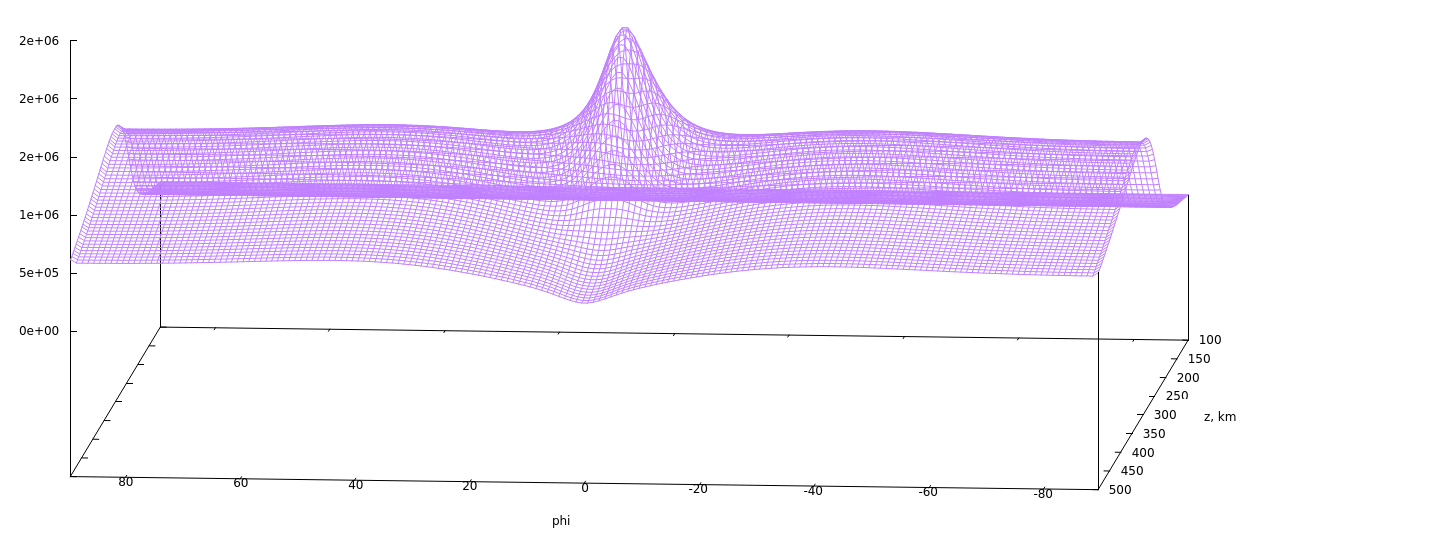
\includegraphics[scale=0.5]{no_mixed_bad_boundary}

Заменим граничное условие: по-прежнему зануляем $A(\varphi_{j-1/2})$, но вместо обнуления компоненты потока, связанной с дивергентным членом, заметим, что точки $-89{,}5^\circ$ и $-90{,}5^\circ$ симметричны, поэтому можно положить требуемое $B(\varphi_{j-1})n_{j-1}$ равным $B(\varphi_j) n_{j}$. После такой замены получим следующую картину: 

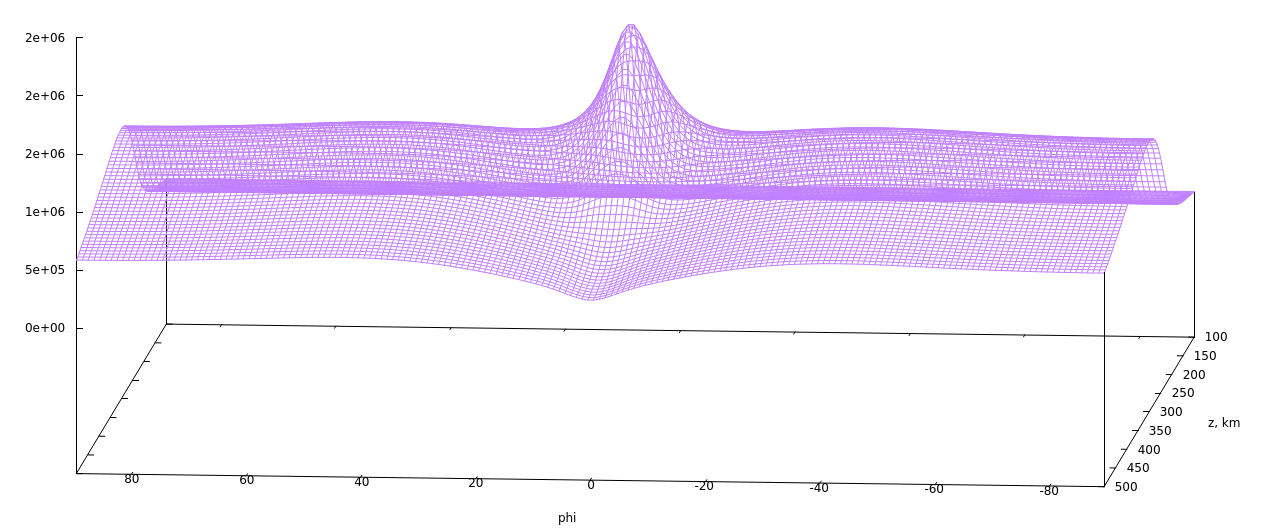
\includegraphics[scale=0.5]{no_mixed_good_boundary}



\begin{center} {\Large Аппроксимации смешанной производной и граничные условия.} \end{center}

Рассмотрим различные аппроксимации для смешанной производной, а также граничные условия в околополюсных точках в уравнении $$\dfrac{\partial n}{\partial t} = \dfrac{1}{a\cos\varphi} \dfrac{\partial }{\partial \varphi}\left[\dfrac{D}{a}\cdot(\cos^2  I \cos\varphi)\cdot\dfrac{\partial n}{\partial \varphi}-D\cdot(\sin I\cos I\cos\varphi)\cdot \dfrac{\partial n}{\partial z} - u\cdot(\sin I \cos I \cos\varphi)\cdot n \right] = $$ $$ =\dfrac{1}{\cos\varphi} \dfrac{\partial }{\partial \varphi}\left[\dfrac{D}{a^2}A(\varphi)\dfrac{\partial n}{\partial \varphi}-\dfrac{D}{2a}B(\varphi) \dfrac{\partial n}{\partial z} - \dfrac{u}{2a}B(\varphi) n \right].$$



\bigskip

{\bf I.} Нелинейная схема. Вводим эффективную скорость $u_z = B(\varphi)\dfrac{1}{n}\dfrac{\partial n}{\partial z} = B(\varphi)\dfrac{\partial \ln n}{\partial z}$. При численном моделировании полагаем $$u_{z(i, j)} \approx B(\varphi)\dfrac{2}{n_{i+1, j}^t+n_{i-1, j}^t}\begin{cases}\dfrac{n_{i+1, j}^t-n_{i, j}^t}{h}, B(\varphi) \geq 0\\\dfrac{n_{i, j}^t-n_{i-1, j}^t}{h}, B(\varphi) \leq 0 .\end{cases}$$ 

После вычисления $u_{z(i, j)}$ в узле $(i, j)$ по значениям $n^t$ с предыдущего временного шага $t$ в зависимости от знака $u_{z(i, j)}$ аппроксимируется смешанная производная: $$-\dfrac{D}{2a\cos\varphi}\dfrac{\partial}{\partial\varphi}\left[u_z n\right] \approx \begin{cases}-\dfrac{D}{2a\cos\varphi_j}\dfrac{u_{z(i, j+1)}n_{i, j+1}^{t+1} - u_{z(i, j)}n_{i, j}^{t+1}}{\Delta\varphi}, u_{z(i, j)} \geq 0\\-\dfrac{D}{2a\cos\varphi_j}\dfrac{u_{z(i, j)}n_{i, j}^{t+1} - u_{z(i, j-1)}n_{i, j-1}^{t+1}}{\Delta\varphi}, u_{z(i, j)} \leq 0.\end{cases}$$

В околополюсных точках $j = 1$ и $j = N_\varphi$ для исключения требуемых в расчете значений вне сетки используем свойства функций $A$ и $B$:

\begin{itemize}
\item[$j = 1$.] В этом случае $A\left(\varphi - \dfrac{\Delta\varphi}{2}\right) = 0$ в точности. Заметим далее, что значение $B(\varphi - \Delta\varphi) n_{i, j-1}$ совпадает с $B(\varphi) n_{i, j}$, эти точки симметричны относительно вертикальной оси. Такое замечание справедливо, когда рассматривается стационарная задача, отвечающая дневному значению фотоионизации и рекомбинации. Для смешанной производной используем тот же приём: в тех случаях, когда требуется вычислить $u_{z(i, j-1)}n_{i, j-1}$, это значение заменяется на равное ему $u_{z(i, j)}n_{i, j}$.

\item[$j = N_\varphi$] Аналогично, $A\left(\varphi + \dfrac{\Delta\varphi}{2}\right) = 0$, а $B(\varphi + \Delta\varphi)n_{i, j+1}$ и $u_{z(i, j+1)}n_{i, j+1}$ заменяются соответственно на $B(\varphi)n_{i, j}$ и $u_{z(i, j)}n_{i, j}$.
\end{itemize}

Результаты расчетов показывают, что имеет место несогласованность такой аппроксимации: возникают ложные источники на границах, похожие на наблюдаемые в схеме без смешанной производной при попытке аппроксимировать полный поток в околополюсной точке нулём.

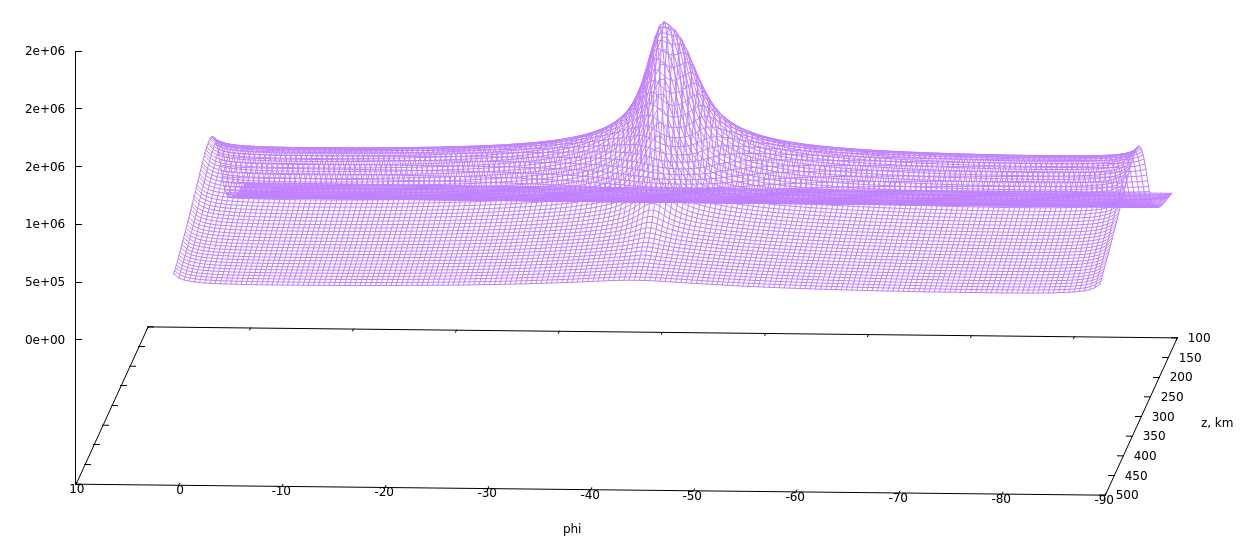
\includegraphics[scale=0.5]{nonlinear}

\bigskip

\newpage



{\bf II.} Линейные схемы первого порядка. Для смешанной производной $-\dfrac{D}{2a\cos\varphi}\dfrac{\partial}{\partial\varphi}\left(B(\varphi)\dfrac{\partial n}{\partial z}\right)$ можно рассмотреть следующие четыре аппроксимации (здесь $B_j \equiv B(\varphi_j)$: 

$$-\dfrac{D}{2a\cos\varphi}\dfrac{\partial}{\partial\varphi}\left(B(\varphi)\dfrac{\partial n}{\partial z}\right) \approx $$ $$\approx-\dfrac{D}{2ah\Delta\varphi \cos\varphi_j} \begin{cases}  B_{j+1} n_{i, j+1}^{t+1} - B_jn_{i, j}^{t+1} - B_{j+1}n_{i-1, j+1}^t + B_j n_{i-1, j}^t \mbox{, справедливо при } B(\varphi_j) < 0 \mbox{, схема (1);}\\ B_{j+1}n_{i+1, j+1}^t - B_j n_{i+1, j}^t - B_{j+1}n_{i, j+1}^{t+1}+B_j n_{i, j}^{t+1}\mbox{, справедливо при } B(\varphi_j) > 0 \mbox{, схема (2);} \\ B_j n_{i,j}^{t+1} - B_{j-1}n_{i, j-1}^{t+1} - B_j n_{i-1, j}^t + B_{j-1}n_{i-1, j-1}^t\mbox{, справедливо при } B(\varphi_j) > 0 \mbox{, схема (3);} \\ B_{j+1}n_{i+1, j+1}^t - B_j n_{i+1, j}^t - B_{j+1}n_{i, j+1}^{t+1} + B_{j}n_{i, j}^{t+1}\mbox{, справедливо при } B(\varphi_j) < 0 \mbox{, схема (4).}\end{cases}$$ 

Первый вариант схемы первого порядка: при $B(\varphi) \geq 0$ (т.~е. в верхнем полушарии) вычисление ведется по формуле (3), а в нижнем полушарии, при $B(\varphi) \leq 0$, соответственно, по формуле (1).

При этом оказывается, что на полюсах разности направлены так, что для вычисления следующего временного слоя не требуется информации о точках вне расчетной области на предыдущем шаге. Поэтому граничные условия в околополюсных точках достаточно применить для слагаемых, отвечающих диффузии и переносу: используются те же условия, что и в предыдущей схеме: на южном полюсе $A\left(\varphi - \dfrac{\Delta\varphi}{2}\right) = 0$, а $B(\varphi - \Delta\varphi) n_{i, j-1}$ заменяется на $B(\varphi) n_{i, j}$. На северном полюсе условия аналогичны.


Второй вариант схемы первого порядка: при $B(\varphi) \geq 0$ (т.~е. в верхнем полушарии) вычисление ведется по формуле (2), а в нижнем полушарии, при $B(\varphi) \leq 0$, соответственно, по формуле (4).

Граничные условия в околополюсных точках для слагаемых, отвечающих диффузии и переносу те же условия, что и в предыдущей схеме. В этой схеме требуются также и значения вне расчетной области для вычисления смешанных производных. Применяем тот же метод: при необходимости вычислить $B_{j+1} n_{i, j+1}$ на северном полюсе заменяем это слагаемое на $B_{j} n_{i, j}$.

Оба варианта вновь показывают несогласованную аппроксимацию вблизи полюсов:

Результаты расчета по первому варианту схемы:

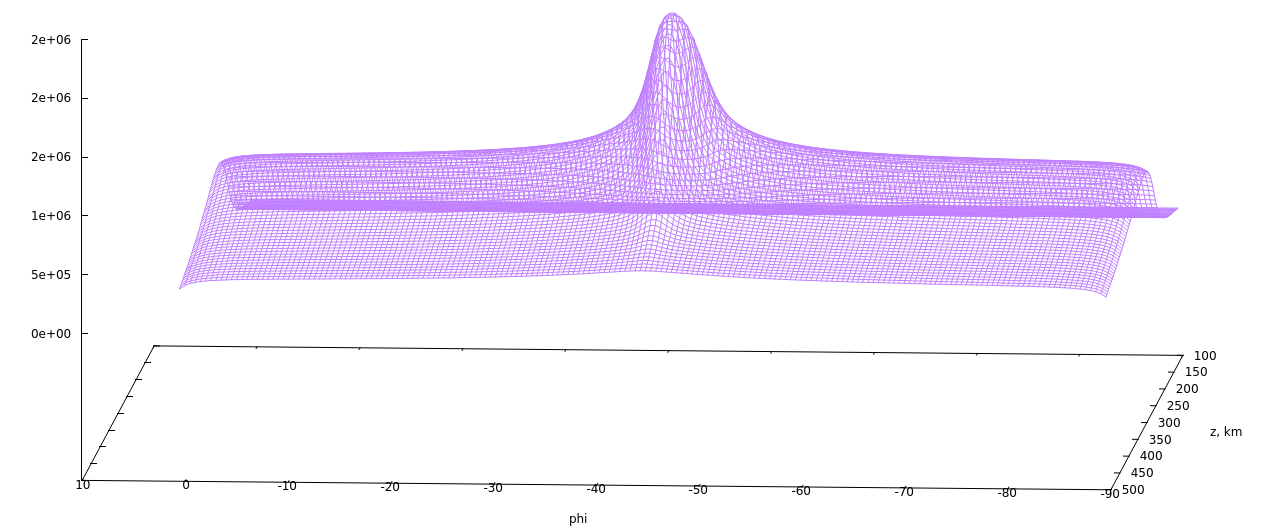
\includegraphics[scale=0.5]{linear_1st_order_1}

Результаты расчета по второму варианту схемы:

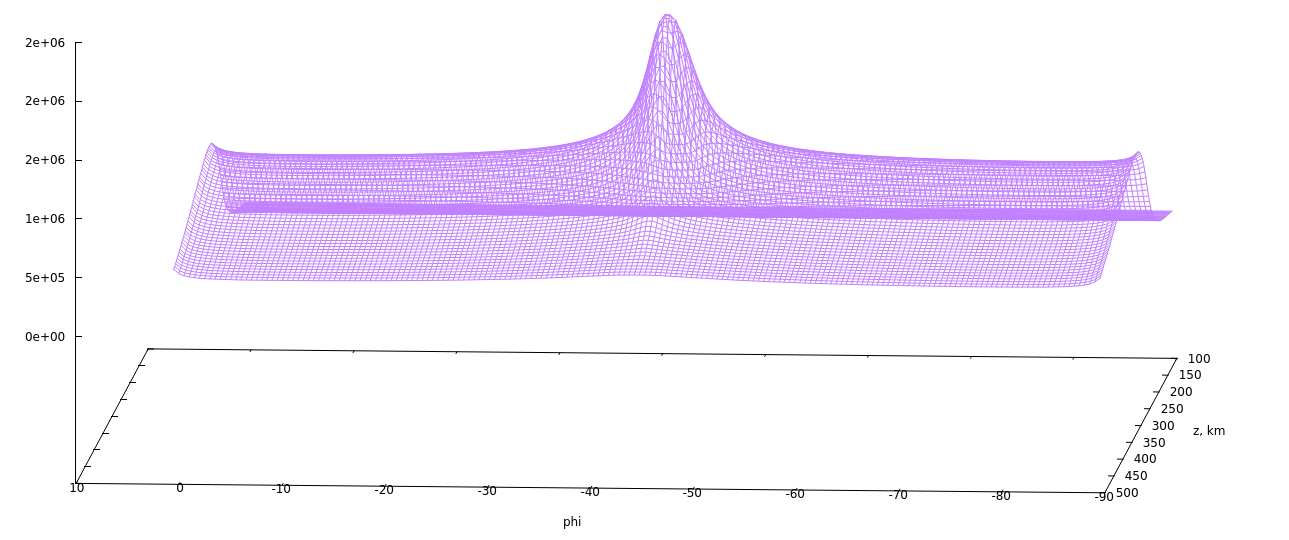
\includegraphics[scale=0.5]{linear_1st_order_2}

\newpage



{\bf III.} Линейная схема второго порядка. Для получения такой схемы используем аппроксимации, рассмотренные в предыдущем пункте: если $B(\varphi) \geq 0$, то аппроксимируем смешанную производную полусуммой аппроксимаций (2) и (3), иначе~---~полусуммой (1) и (4). Для вычисления в околополюсных точках вновь отождествляем необходимые точки вне расчетной области с симметричными им относительно полюсов. На этот раз такая аппроксимация согласована: 

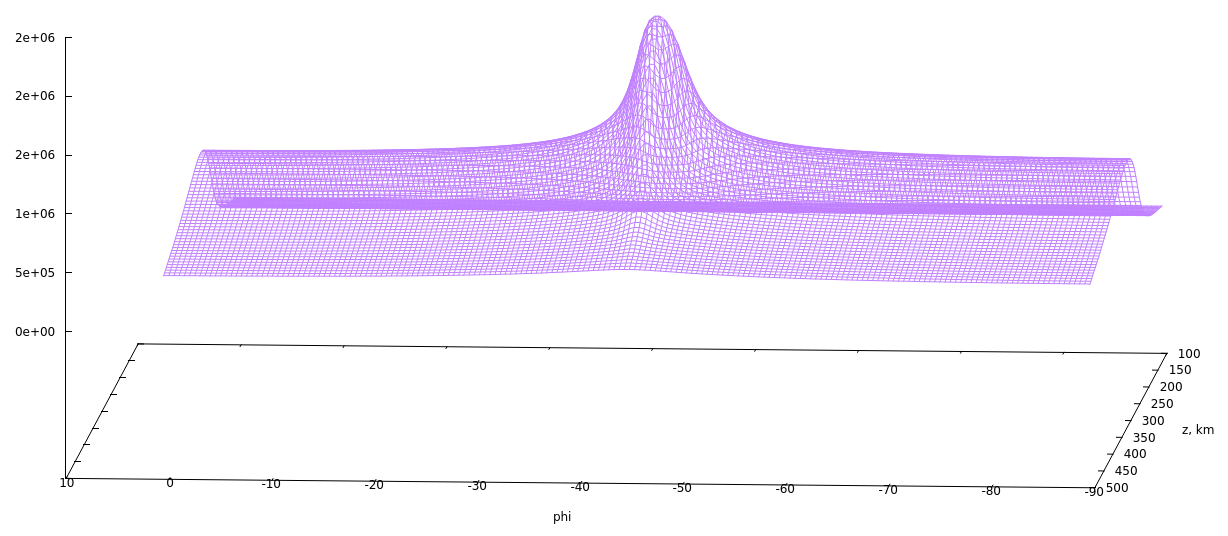
\includegraphics[scale=0.5]{linear_2st_order}

\end{document}



